\vspace*{10mm}
\setlength{\TPHorizModule}{10pt}
\setlength{\TPVertModule}{10pt}
\begin{textblock}{1}(43.25,15.75) % Photo is adusted flush to the right margin - SBÖ
	\begin{figure}[p]
		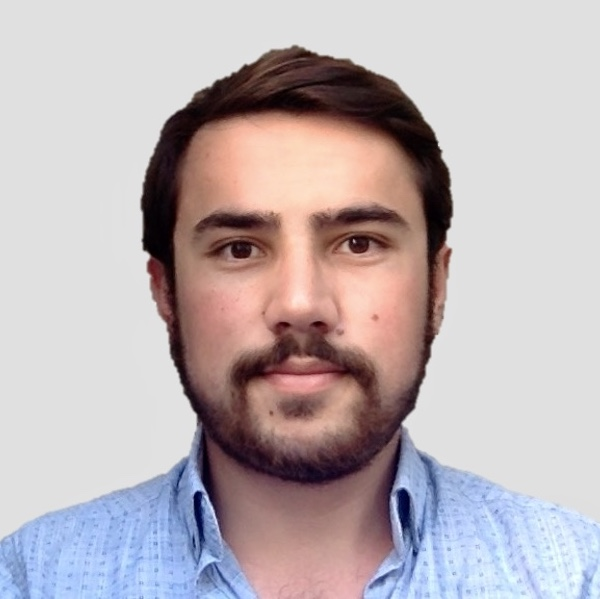
\includegraphics[scale=0.15,keepaspectratio=true]{Picture2_600by600.jpg}
	\end{figure}	
\end{textblock}
\vspace*{30mm}
\textbf{Name Surname\makebox[2.155cm]{\hfill \textbf{:}}}\hspace{0.225em} Ahmet Oğuz Güzel\\ % Adjust the colomn alignment - SBÖ

\vspace{-3mm}
\textbf{Place and Date of Birth\makebox[0.735cm]{\hfill \textbf{:}}}\hspace{0.225em} Turkey, 1995\\ % Adjust the colomn alignment - SBÖ

\vspace{-3mm}
\textbf{E-Mail\makebox[3.685cm]{\hfill \textbf{:}}}\hspace{0.225em} guzelah@itu.edu.tr\\ % Adjust the colomn alignment - SBÖ

\vspace{5mm}

\renewcommand\labelitemi{\normalsize$\bullet$} 			% Adjust the size of the bullets - SBÖ

\textbf{EDUCATION\makebox[2.41cm]{\hfill \textbf{}}}  	% Adjust the column alignment - SBÖ
\vspace{-3mm}

\begin{itemize}[leftmargin=5.15cm,itemsep=-0.25em,labelsep=2mm] % Adjust margin to flush left, item sep., label sep. - SBÖ
	\item [$\bullet$ \hspace{1em}\textbf{M.Sc.} \hspace{6.55em} \textbf{:}] 2022, Istanbul Technical University, Graduate School, Department of Physics Engineering, Physics Engineering Programme
	\item [$\bullet$ \hspace{1em}\textbf{B.Sc.} \hspace{6.85em} \textbf{:}] 2019, Istanbul Technical University, Faculty of Aeronautics and Astronautics, Department of Astronautical Engineering
\end{itemize}

\textbf{PROFESSIONAL EXPERIENCE}   
\vspace{-3mm}
\begin{itemize}[leftmargin=0.7cm,itemsep=-0.25em,labelsep=5mm] % Adjust margin to flush left, item sep., label sep. - SBÖ
	%\setlength{\itemindent}{-0.25em}
	\item CMS User, CERN
	\item Associate researcher at the Turkish Atomic Energy Authority, TAEK
\end{itemize}

\textbf{PUBLICATIONS} 
\vspace{-3mm}
\begin{itemize}[leftmargin=0.7cm,itemsep=0.5em,labelsep=5mm] % Adjust margin to flush left, item sep., label seperation - SBÖ
	%\setlength{\itemindent}{-0.25em}
	
	\item \textbf{The ATLAS and CMS Collaborations} 2022. Snowmass White Paper Contribution: Physics with the Phase-2 ATLAS and CMS Detectors, 
	\textit{ATL-PHYS-PUB-2022-018, CMS-PAS-FTR-22-001},
	\href{https://cds.cern.ch/record/2806962?ln=en}{https://cds.cern.ch/record/2806962?ln=en}.
	
	\item \textbf{The CMS Collaboration} 2022. Prospects for HH measurements in the \wwgg and \ttgg final states in proton-proton collisions at $\sqrt{s}=14$ TeV at the HL-LHC, 
	\textit{CMS-PAS-FTR-21-003},
	\href{https://cds.cern.ch/record/2804003?ln=en}{https://cds.cern.ch/record/2804003?ln=en}.

	\item \textbf{Altan Cakir and Oguz Guzel} 2019. A Brief Review of Plasma Wakefield Acceleration, 
	\textit{arXiv,}
	\href{https://arxiv.org/abs/1908.07207}{https://arxiv.org/abs/1908.07207}.

\end{itemize}

%\newpage

%\textbf{GIVEN PRESENTATIONS}
%\vspace{-3mm}
% ---------------------------------------------------------------- %
% Fotografli ve yayin listeli (yayini varsa) ozgecmis onerilir.    %
% Fotograf ve adres sart degildir.				                   %
% ---------------------------------------------------------------- %

%======================================== SIRT OF THE THESIS ========================================= - SBÖ
\newpage % Last page is assigned for the SIRT of the Thesis 
\thispagestyle{empty} % Remove the bottom page number
% Definitions in sırt of the thesis
\def\sirtyili{2022} % Year of the graduation
\def\studentname{A. O. GÜZEL} % F. and M. initials SURNAME
\def\thesisthickness{25mm} % Enter the expected thickness of the thesis after the hardcover 

\hspace*{75mm}
\begin{tikzpicture}[remember picture,overlay]
{\rotatebox[origin=c,x=23.35mm,y=-247.75mm]{90}{\draw [line width=0.01mm, black, dashed] (0mm,0mm) rectangle node{\normalsize \studentname} (65mm,\thesisthickness);}}

{\rotatebox[origin=c,x=23.35mm,y=-247.75mm]{90}{\draw [line width=0.01mm, black ,dashed, text width=190mm, align=center] (67mm,0mm) rectangle node{\normalsize \Baslikspacing \Baslikbir~\Baslikiki~\Baslikuc} (193mm+65mm+2mm,\thesisthickness);}}

{\rotatebox[origin=c,x=23.35mm,y=-247.75mm]{90}{\draw [line width=0.01mm, black ,dashed] (193mm+65mm+4mm,0mm) rectangle node{\normalsize \sirtyili} (296.5mm,\thesisthickness);}}

{\rotatebox[origin=c,x=23.35mm,y=-247.75mm]{90}{\draw[black,line width=1mm] (64.5mm,0mm) -- (64.5mm,\thesisthickness);
\draw[black,line width=1mm] (67.3mm,0mm) -- (67.3mm,\thesisthickness);
}}

{\rotatebox[origin=c,x=23.35mm,y=-247.75mm]{90}{\draw[black,line width=1mm] (193mm+64.5mm+2mm,0mm) -- (193mm+64.5mm+2mm,\thesisthickness);
\draw[black,line width=1mm] (193mm+64.5mm+5mm,0mm) -- (193mm+64.5mm+5mm,\thesisthickness);
}}
% Four dashed lines added between double thick lines vertically
\draw [line width=0.01mm, black, dashed] (0mm,-205mm) -- (0mm,-208mm);
\draw [line width=0.01mm, black, dashed] (-\thesisthickness,-205mm) -- (-\thesisthickness,-208mm);
\draw [line width=0.01mm, black, dashed] (0mm,-3.25mm) -- (0mm,-13mm);
\draw [line width=0.01mm, black, dashed] (-\thesisthickness,-1mm) -- (-\thesisthickness,-13mm);
\end{tikzpicture}